% Options for packages loaded elsewhere
\PassOptionsToPackage{unicode}{hyperref}
\PassOptionsToPackage{hyphens}{url}
\documentclass[
]{book}
\usepackage{xcolor}
\usepackage{amsmath,amssymb}
\setcounter{secnumdepth}{5}
\usepackage{iftex}
\ifPDFTeX
  \usepackage[T1]{fontenc}
  \usepackage[utf8]{inputenc}
  \usepackage{textcomp} % provide euro and other symbols
\else % if luatex or xetex
  \usepackage{unicode-math} % this also loads fontspec
  \defaultfontfeatures{Scale=MatchLowercase}
  \defaultfontfeatures[\rmfamily]{Ligatures=TeX,Scale=1}
\fi
\usepackage{lmodern}
\ifPDFTeX\else
  % xetex/luatex font selection
\fi
% Use upquote if available, for straight quotes in verbatim environments
\IfFileExists{upquote.sty}{\usepackage{upquote}}{}
\IfFileExists{microtype.sty}{% use microtype if available
  \usepackage[]{microtype}
  \UseMicrotypeSet[protrusion]{basicmath} % disable protrusion for tt fonts
}{}
\makeatletter
\@ifundefined{KOMAClassName}{% if non-KOMA class
  \IfFileExists{parskip.sty}{%
    \usepackage{parskip}
  }{% else
    \setlength{\parindent}{0pt}
    \setlength{\parskip}{6pt plus 2pt minus 1pt}}
}{% if KOMA class
  \KOMAoptions{parskip=half}}
\makeatother
\usepackage{color}
\usepackage{fancyvrb}
\newcommand{\VerbBar}{|}
\newcommand{\VERB}{\Verb[commandchars=\\\{\}]}
\DefineVerbatimEnvironment{Highlighting}{Verbatim}{commandchars=\\\{\}}
% Add ',fontsize=\small' for more characters per line
\usepackage{framed}
\definecolor{shadecolor}{RGB}{248,248,248}
\newenvironment{Shaded}{\begin{snugshade}}{\end{snugshade}}
\newcommand{\AlertTok}[1]{\textcolor[rgb]{0.94,0.16,0.16}{#1}}
\newcommand{\AnnotationTok}[1]{\textcolor[rgb]{0.56,0.35,0.01}{\textbf{\textit{#1}}}}
\newcommand{\AttributeTok}[1]{\textcolor[rgb]{0.13,0.29,0.53}{#1}}
\newcommand{\BaseNTok}[1]{\textcolor[rgb]{0.00,0.00,0.81}{#1}}
\newcommand{\BuiltInTok}[1]{#1}
\newcommand{\CharTok}[1]{\textcolor[rgb]{0.31,0.60,0.02}{#1}}
\newcommand{\CommentTok}[1]{\textcolor[rgb]{0.56,0.35,0.01}{\textit{#1}}}
\newcommand{\CommentVarTok}[1]{\textcolor[rgb]{0.56,0.35,0.01}{\textbf{\textit{#1}}}}
\newcommand{\ConstantTok}[1]{\textcolor[rgb]{0.56,0.35,0.01}{#1}}
\newcommand{\ControlFlowTok}[1]{\textcolor[rgb]{0.13,0.29,0.53}{\textbf{#1}}}
\newcommand{\DataTypeTok}[1]{\textcolor[rgb]{0.13,0.29,0.53}{#1}}
\newcommand{\DecValTok}[1]{\textcolor[rgb]{0.00,0.00,0.81}{#1}}
\newcommand{\DocumentationTok}[1]{\textcolor[rgb]{0.56,0.35,0.01}{\textbf{\textit{#1}}}}
\newcommand{\ErrorTok}[1]{\textcolor[rgb]{0.64,0.00,0.00}{\textbf{#1}}}
\newcommand{\ExtensionTok}[1]{#1}
\newcommand{\FloatTok}[1]{\textcolor[rgb]{0.00,0.00,0.81}{#1}}
\newcommand{\FunctionTok}[1]{\textcolor[rgb]{0.13,0.29,0.53}{\textbf{#1}}}
\newcommand{\ImportTok}[1]{#1}
\newcommand{\InformationTok}[1]{\textcolor[rgb]{0.56,0.35,0.01}{\textbf{\textit{#1}}}}
\newcommand{\KeywordTok}[1]{\textcolor[rgb]{0.13,0.29,0.53}{\textbf{#1}}}
\newcommand{\NormalTok}[1]{#1}
\newcommand{\OperatorTok}[1]{\textcolor[rgb]{0.81,0.36,0.00}{\textbf{#1}}}
\newcommand{\OtherTok}[1]{\textcolor[rgb]{0.56,0.35,0.01}{#1}}
\newcommand{\PreprocessorTok}[1]{\textcolor[rgb]{0.56,0.35,0.01}{\textit{#1}}}
\newcommand{\RegionMarkerTok}[1]{#1}
\newcommand{\SpecialCharTok}[1]{\textcolor[rgb]{0.81,0.36,0.00}{\textbf{#1}}}
\newcommand{\SpecialStringTok}[1]{\textcolor[rgb]{0.31,0.60,0.02}{#1}}
\newcommand{\StringTok}[1]{\textcolor[rgb]{0.31,0.60,0.02}{#1}}
\newcommand{\VariableTok}[1]{\textcolor[rgb]{0.00,0.00,0.00}{#1}}
\newcommand{\VerbatimStringTok}[1]{\textcolor[rgb]{0.31,0.60,0.02}{#1}}
\newcommand{\WarningTok}[1]{\textcolor[rgb]{0.56,0.35,0.01}{\textbf{\textit{#1}}}}
\usepackage{longtable,booktabs,array}
\usepackage{calc} % for calculating minipage widths
% Correct order of tables after \paragraph or \subparagraph
\usepackage{etoolbox}
\makeatletter
\patchcmd\longtable{\par}{\if@noskipsec\mbox{}\fi\par}{}{}
\makeatother
% Allow footnotes in longtable head/foot
\IfFileExists{footnotehyper.sty}{\usepackage{footnotehyper}}{\usepackage{footnote}}
\makesavenoteenv{longtable}
\usepackage{graphicx}
\makeatletter
\newsavebox\pandoc@box
\newcommand*\pandocbounded[1]{% scales image to fit in text height/width
  \sbox\pandoc@box{#1}%
  \Gscale@div\@tempa{\textheight}{\dimexpr\ht\pandoc@box+\dp\pandoc@box\relax}%
  \Gscale@div\@tempb{\linewidth}{\wd\pandoc@box}%
  \ifdim\@tempb\p@<\@tempa\p@\let\@tempa\@tempb\fi% select the smaller of both
  \ifdim\@tempa\p@<\p@\scalebox{\@tempa}{\usebox\pandoc@box}%
  \else\usebox{\pandoc@box}%
  \fi%
}
% Set default figure placement to htbp
\def\fps@figure{htbp}
\makeatother
\setlength{\emergencystretch}{3em} % prevent overfull lines
\providecommand{\tightlist}{%
  \setlength{\itemsep}{0pt}\setlength{\parskip}{0pt}}
\usepackage[]{natbib}
\bibliographystyle{plainnat}
\usepackage{booktabs}
\usepackage{bookmark}
\IfFileExists{xurl.sty}{\usepackage{xurl}}{} % add URL line breaks if available
\urlstyle{same}
\hypersetup{
  pdftitle={Descriptive Statistics for Two Variables},
  pdfauthor={Samuel Rowe adapted from Acock (2023)},
  hidelinks,
  pdfcreator={LaTeX via pandoc}}

\title{Descriptive Statistics for Two Variables}
\author{Samuel Rowe adapted from Acock (2023)}
\date{2026-08-23}

\begin{document}
\maketitle

{
\setcounter{tocdepth}{1}
\tableofcontents
}
\begin{Shaded}
\begin{Highlighting}[]
\NormalTok{bookdown}\SpecialCharTok{::}\FunctionTok{render\_book}\NormalTok{()}
\end{Highlighting}
\end{Shaded}

\chapter*{Overview}\label{overview}
\addcontentsline{toc}{chapter}{Overview}

Topics:

\begin{enumerate}
\def\labelenumi{\arabic{enumi}.}
\tightlist
\item
  Descriptive Statistics for Two Variables
\item
  Exercises
\end{enumerate}

\chapter{Descriptive Statistics for Two Variables}\label{descriptive-statistics-for-two-variables}

At the end of last week, we began examine the relationship between variables. We split hours spent on the internet by sex. We were examining how hours varied between two groups, even though we were focusing on the descriptive statistics for one variable,

Providing descriptive statistics is an essential part of any study. Before you can look at relationships, you need to describe the data: central tendency, variability, and distribution. However, we want to see how descriptive statistics may vary between two variables.

Before more rigorous studies are conducted, researchers conduct descriptive analyses to see if there are associations between two variables. We will start to dive into the statistical methods to look for associations or relationshps between two variables.

Many research questions stem from the association between two variables

\begin{enumerate}
\def\labelenumi{\arabic{enumi}.}
\tightlist
\item
  Do women who are drug dependent us different drugs from those used by drug-dependent men?
\item
  Are women more likely to be progressive than men?
\item
  Is there a relationship between religiosity and support for increased spending on public health?
\item
  Is there an association between a training program and long-term wages?
\item
  Is a school intervention lead to higher rates of graduation?
\end{enumerate}

We will learn how to describe relationship between categorical variables from this chapter. What are our tests? What are the potential problems with the test? What are possible misinterpretations?

Acock (2023) tells us that the best statistics are the simplest statistics to use. Honestly, I agree. As we go through the empirical sequence, you will learn more sophisticated but the begin to tradeoff simplicity for rigor. This comes a cost of fewer people understanding your methods.

One of the simplest methods is the two-way tabulation or cross-tabulation. We can examine any potential relationship between two categorical with a \(\chi^2\) test within a two-way tabulation or cross-tabulation.

\section{Crosstabulation or two-way tabulations}\label{crosstabulation-or-two-way-tabulations}

A two-way tabulation or cross-tabulation is a table of rows representing on categorical variable and columns representing another categorical variable. These tables are also sometimes called contigency tables, since response maybe contingent on another variable. For example, support for a particular policy may be contigent on someone's demographics, such as sex.

Acock (2023) starts off with looking at cross-tabulations between abortion opinions and sex from the 2006 General Social Survey. We have two categorical variables, \emph{sex} and \emph{abany}. We will use sex as the row and abortion opinion as the columns. For the \emph{tabulate} or \emph{tab } command, the first variable after the work \emph{tabulate} is the row variable and the second is the column variable.

We will use \emph{sex} as the explanatory variable and \emph{abany} as the outcome or dependent variable. We want to explain someone's opinion on abortion by sex. Please note that explanatory variable may be called independent variables, explanatory variables, or predictor variables.

Note: Acock (2023) brings up a good point about independent and dependent variables. Can dependent variable influence the independent variable? Pay attention to this, because you will delve more into this during Econ 645. This is also way it is essential to start with a research question and then use economic theory before using statistical methods. There could be a third variable that influences both the dependent and independent variable, which makes it look like there is a relationship when there isn't any. E.g.: There is an association between shark attacks and ice cream. However, once we understand the summer time is associated with both shark attacks and ice cream consumption, the spurious relationship dissolves.

\begin{Shaded}
\begin{Highlighting}[]
\NormalTok{cd }\StringTok{"/Users/Sam/Desktop/Econ 643/Data/agis6r/"}
\KeywordTok{use}\NormalTok{ gss2006\_chapter6, }\KeywordTok{clear}
\KeywordTok{tabulate}\NormalTok{ sex abany}
\end{Highlighting}
\end{Shaded}

\begin{verbatim}
/Users/Sam/Desktop/Econ 643/Data/agis6r

(General Social Surveys, 1972-2006 [Cumulative File], Dataset 0001)

           |   ABORTION IF WOMAN
           | WANTS FOR ANY REASON
    GENDER |       YES         NO |     Total
-----------+----------------------+----------
      MALE |       350        478 |       828 
    FEMALE |       434        677 |     1,111 
-----------+----------------------+----------
     Total |       784      1,155 |     1,939 
\end{verbatim}

350 out of 828 males reported it is okay to have an abortion for any reason, while 434 out of 1,111 women said the same.

After looking over this result, it is hard to tell if there are differences in opinion between men and women. We can look at the within-row frequencies, but it is hard to compare. Let's look at \textbf{conditional probability}. What is \(P(Y|M)\) or what is the probability of saying yes given the individual is a male? What is \(P(N|W)\) or what is the probability of saying no when the individual is a male?

\begin{Shaded}
\begin{Highlighting}[]
\KeywordTok{tabulate}\NormalTok{ sex abany, }\OtherTok{row}
\end{Highlighting}
\end{Shaded}

\begin{verbatim}
| Key            |
|----------------|
|   frequency    |
| row percentage |
+----------------+

           |   ABORTION IF WOMAN
           | WANTS FOR ANY REASON
    GENDER |       YES         NO |     Total
-----------+----------------------+----------
      MALE |       350        478 |       828 
           |     42.27      57.73 |    100.00 
-----------+----------------------+----------
    FEMALE |       434        677 |     1,111 
           |     39.06      60.94 |    100.00 
-----------+----------------------+----------
     Total |       784      1,155 |     1,939 
           |     40.43      59.57 |    100.00 
\end{verbatim}

Interestingly, a higher percentage of males say it is okay to have an abortion for any reason at 42.3\% compared to women at 39.1\%. It is a small difference, so it makes us wonder if the result is statistically significant. In order to find out, we will use a \(\chi^2\) test.

\section{\texorpdfstring{\(\chi^2\) test}{\textbackslash chi\^{}2 test}}\label{chi2-test}

How can we say there is a relationship between sex and opinion on abortion? Is this by chance? Is it an actual relationship? Is the difference statistically significant? Maybe our \(N\) is large enough to find any difference is statistically significant.

We will set up a null hypothesis that there is no difference between men and women for abortion opinions.

\(H_0:\) There is no difference between men and women.

\(H_A:\) There is a difference between men and women.

We will use a \(\chi^2\) test to test the likelihood that the result occurred by chance. The \(\chi^2\) test compares the frequency in each cell with what you would expect if there were no relationship. The expected frequency depends upon how many people are in the rows and columns.

We will add three additional options to our \emph{tabulate} command to test the relationship between \emph{sex} and \emph{abany}. We will add \emph{row} to look for conditional probability. We will add \emph{expected} to add the expected frequency if there were no relationship. Also, we will add \emph{chi2} to conduct a \(\chi^2\) test. We can add \emph{cchi2} to look at the contributions toward \(\chi^2\).

\begin{Shaded}
\begin{Highlighting}[]
\KeywordTok{tabulate}\NormalTok{ sex abany, }\OtherTok{row}
\end{Highlighting}
\end{Shaded}

\begin{verbatim}
| Key                |
|--------------------|
|     frequency      |
| expected frequency |
| chi2 contribution  |
|   row percentage   |
+--------------------+

           |   ABORTION IF WOMAN
           | WANTS FOR ANY REASON
    GENDER |       YES         NO |     Total
-----------+----------------------+----------
      MALE |       350        478 |       828 
           |     334.8      493.2 |     828.0 
           |       0.7        0.5 |       1.2 
           |     42.27      57.73 |    100.00 
-----------+----------------------+----------
    FEMALE |       434        677 |     1,111 
           |     449.2      661.8 |   1,111.0 
           |       0.5        0.3 |       0.9 
           |     39.06      60.94 |    100.00 
-----------+----------------------+----------
     Total |       784      1,155 |     1,939 
           |     784.0    1,155.0 |   1,939.0 
           |       1.2        0.8 |       2.0 
           |     40.43      59.57 |    100.00 

          Pearson chi2(1) =   2.0254   Pr = 0.155
\end{verbatim}

Within each cell, we have the frequency, the expected frequency, the \(\chi^2\) contribution, and the conditional probability. The expected frequency is calculated by the marginal frequencies of the row by the maringal frequency of the column divided by the total.

\[ (Total Men * Total Yes)/Total = Expected Frequency for Men and Yes \]

For our upper left cell:

\[ (784*828)/1,939 = 334.8 \]

\begin{figure}
\centering
\pandocbounded{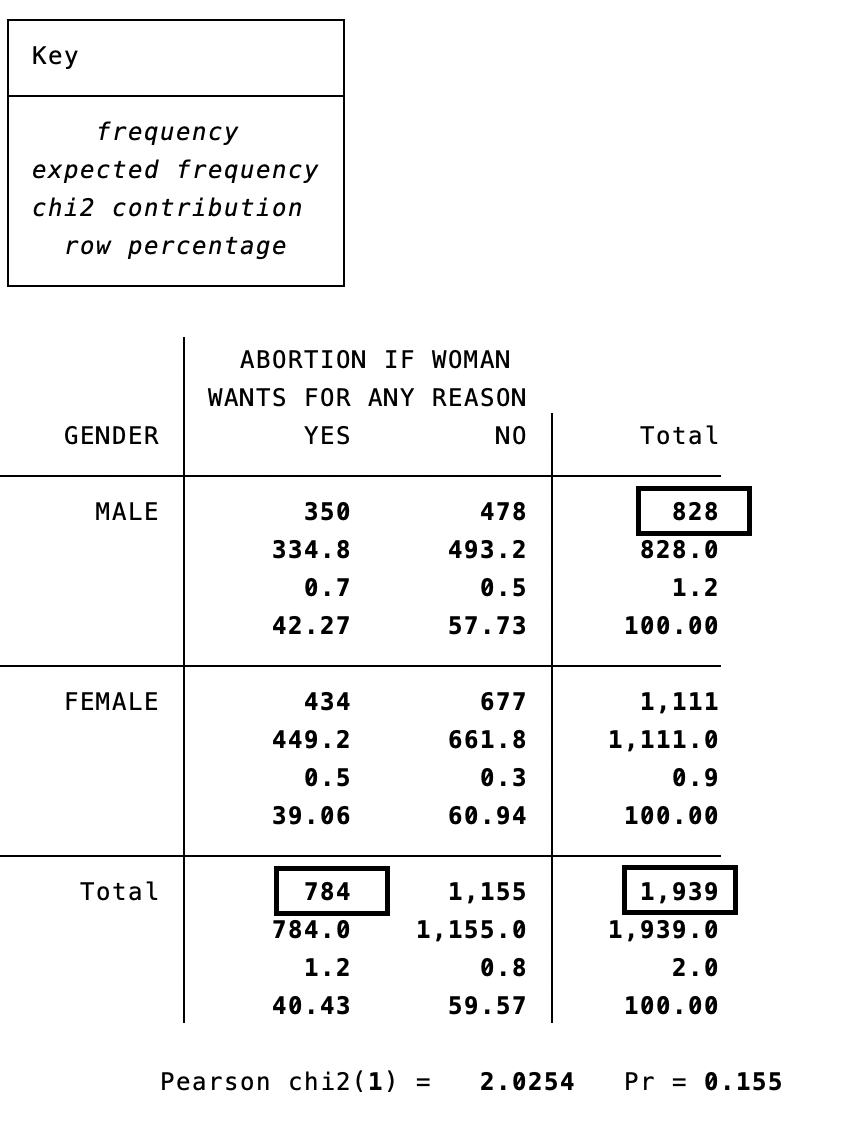
\includegraphics[keepaspectratio,alt={Figure 4.1: Expected Frequency Calculation}]{week4_expected.png}}
\caption{Figure 4.1: Expected Frequency Calculation}
\end{figure}

\[ \]

We calculate the \(\chi_2\) as the following:

\[ \chi_2 = \sum \frac{(O_i-E_i)^2 }{E_i} \]

Each the statistic for each \textbf{joint frequency} \(i\). Such that, for the upper left cell:

\[ \frac{(350-334.8)^2}{334.8}=0.7 \]
And we calculate \(\chi^2\) as \(\chi^2 = 0.7+0.5+0.5+0.3=2.0\)

We compare our \(\chi^2\) statistic to a \(\chi^2\) distribution. Before we go to the \(\chi^2\) distribution, we need to get the \textbf{degrees of freedom}. Our degrees of freedom can be calculated as the number of rows minus 1 times the number of columns minus 1:

\[ df=(R-1)\times(C-1) \]

This means that we have one degree of freedom \((2-1)\times(2-1)=1\).

Next, we need to get our \textbf{critical value} to compare. We will set our \(\alpha=0.05\) or a 95\% confidence level. Using this, we can go to a \(\chi^2\) distribution to get our critical value to compare to our \(\chi^2\) statistic.

\begin{figure}
\centering
\pandocbounded{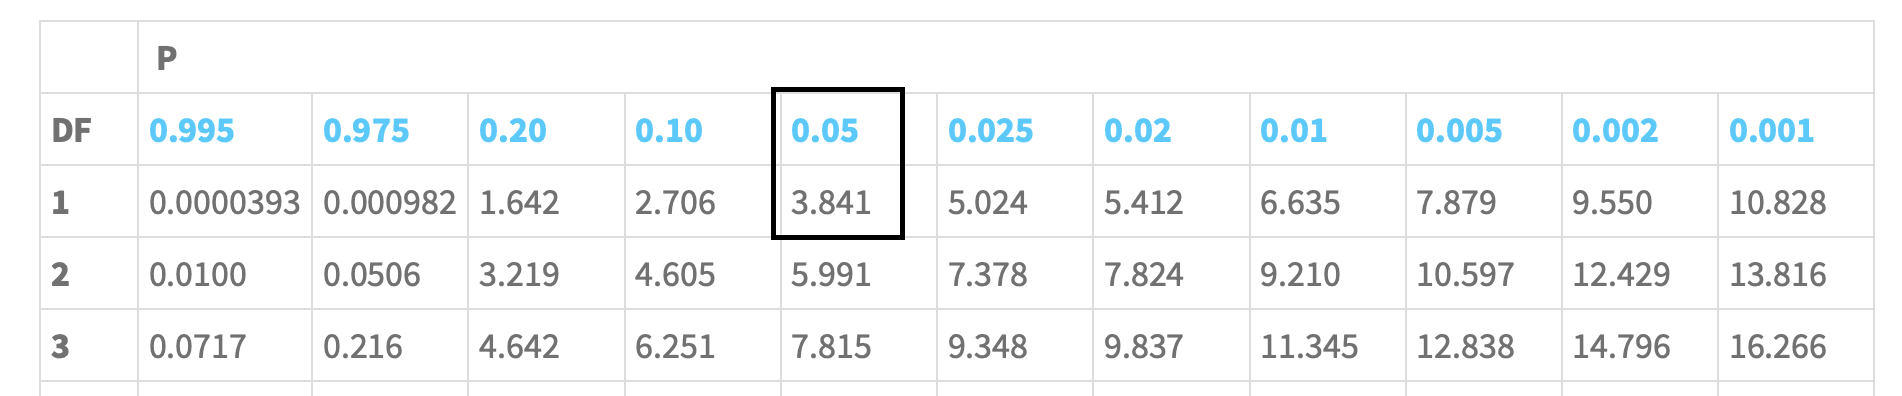
\includegraphics[keepaspectratio,alt={Figure 4.2: \textbackslash chi\^{}2 table}]{week4_chi2table.png}}
\caption{Figure 4.2: \(\chi^2\) table}
\end{figure}

\[ \]

Next, we will compare our \(\chi^2=2.02\) to the critical value of \(3.841\). Since \(2.02 < 3.841\), we fail to reject the null hypothesis that there is no difference in abortion opinions between men and women at the 95\% confidence level. We can also look at the \(p\)-value where \(p = 0.155\) where \(p > 0.05\), which means we fail to reject the null hypothesis at the 5\% level.

As a side note, we can use Stata to get the \(\chi^2\) table.

\begin{Shaded}
\begin{Highlighting}[]
\KeywordTok{search}\NormalTok{ chitable}
\end{Highlighting}
\end{Shaded}

After installing the package probtabl, you can get a \(\chi^2\) table by typing \emph{chitable 1} for the \(\chi^2\) table with 1 degree of freedom:

\begin{Shaded}
\begin{Highlighting}[]
\NormalTok{chitable 1}
\end{Highlighting}
\end{Shaded}

\begin{verbatim}
        Critical Values of Chi-square
 df     .50     .25     .10     .05    .025      .01     .001
  1    0.45    1.32    2.71    3.84    5.02     6.63    10.83
\end{verbatim}

\section{Measures of Association}\label{measures-of-association}

We need to be wary when we find statistical significance with large samples. Even weak relationship may appear to be significant. Our \(\chi^2\) depends upon the relationship between two variables and the sample size.

We can utilize Cramer's \(V\) to prevent misinterpreting a relationship when one does not exist. We can account for the sample size with Cramer's \(V\) with the following formula:

\[ V=\sqrt{ \frac{\chi^2}{N \times min(R-1,C-1)}} \]
\(V\) will be bound between 0 and 1. A Cramer's \(V\) between 0 and 0.19 is considered weak, while a value between 0.20 and 0.49 is considered moderate. A value of 0.5 or more is considered strong. Cramer's V looks for the relationship instead of statistical significance. Please note that \(V\) can be negative due to the order of the columns, so it is really bound between -1 and +1 with 0 showing no relationship.

We need to add the option \emph{V} in \emph{tabulate} to calculate Cramer's \(V\) in Stata.

\begin{Shaded}
\begin{Highlighting}[]
\KeywordTok{tabulate}\NormalTok{ sex abany, }\FunctionTok{chi2} \OtherTok{row} \KeywordTok{V}
\end{Highlighting}
\end{Shaded}

\begin{verbatim}
| Key            |
|----------------|
|   frequency    |
| row percentage |
+----------------+

           |   ABORTION IF WOMAN
           | WANTS FOR ANY REASON
    GENDER |       YES         NO |     Total
-----------+----------------------+----------
      MALE |       350        478 |       828 
           |     42.27      57.73 |    100.00 
-----------+----------------------+----------
    FEMALE |       434        677 |     1,111 
           |     39.06      60.94 |    100.00 
-----------+----------------------+----------
     Total |       784      1,155 |     1,939 
           |     40.43      59.57 |    100.00 

          Pearson chi2(1) =   2.0254   Pr = 0.155
               Cramér's V =   0.0323
\end{verbatim}

Our result shows a weak relationship between sex and opinion on abortion.

We can use a data set from the Steering Commitee of the Physicians' Health Study Research Group. This data set looks at the relationship between men and taking daily aspirin.

\begin{Shaded}
\begin{Highlighting}[]
\KeywordTok{use}\NormalTok{ chapter6\_aspirin, }\KeywordTok{clear}
\KeywordTok{tabulate}\NormalTok{ aspirin heartattack, }\FunctionTok{chi2} \OtherTok{row} \KeywordTok{V}
\end{Highlighting}
\end{Shaded}

\begin{verbatim}
| Key            |
|----------------|
|   frequency    |
| row percentage |
+----------------+

           |     Heart Attack
 Condition | No Attack     Attack |     Total
-----------+----------------------+----------
   Placebo |    10,845        189 |    11,034 
           |     98.29       1.71 |    100.00 
-----------+----------------------+----------
   Aspirin |    10,933        104 |    11,037 
           |     99.06       0.94 |    100.00 
-----------+----------------------+----------
     Total |    21,778        293 |    22,071 
           |     98.67       1.33 |    100.00 

          Pearson chi2(1) =  25.0139   Pr = 0.000
               Cramér's V =  -0.0337
\end{verbatim}

We can see that we reject the null hypothesis at the 5\% level (even the 0.1\% level) from the \(\chi^2\) test. However, when we look at Cramer's \(V\) we see two things. One the value is negative and the value is near 0. The order of the column matter is the value is negative or positive, but the main take away is the relationship is weak.

\section{Ordinal Categorical Variables}\label{ordinal-categorical-variables}

We can test the relationship between two ordinal variables. We will look at \emph{health} and \emph{happy} for how respondents reported their health and happiness, respectively, in the 2006 General Social Survey. We will set health as the explanatory or independent variable and happiness as the outcome or dependent variable.

We need to introduce two additional tests besides a \(\chi^2\) test and Cramer's \(V\) when variables of interest of ordinal. We will introduce Goodman and Kruskal's \(\gamma\) and Kendall's \(\tau_{b}\). Both \(\gamma\) and \(\tau_{b}\) are measures of association for ordinal data. If one person is happier, then we expect them to be healthier, as well. \(\tau_b\) is close to a correlation coefficient. Such that, a \(\tau_b\) less than 0.2 shows a weak relationship, while a \(\tau_b\) between 0.2 and 0.49 shows a moderate relationship. A \(\tau_b\) of 0.5 or above indicate a strong relationship.

In Stata, all we need to do is add the options \emph{gamma} and \emph{taub} to our \emph{tabulate} command.

\begin{Shaded}
\begin{Highlighting}[]
\KeywordTok{use}\NormalTok{ gss2006\_chapter6, }\KeywordTok{clear}
\KeywordTok{tabulate}\NormalTok{ health happy, }\FunctionTok{chi2}\NormalTok{ column }\KeywordTok{gamma} \OtherTok{row}\NormalTok{ taub }\KeywordTok{V}
\end{Highlighting}
\end{Shaded}

\begin{verbatim}
(General Social Surveys, 1972-2006 [Cumulative File], Dataset 0001)


+-------------------+
| Key               |
|-------------------|
|     frequency     |
|  row percentage   |
| column percentage |
+-------------------+

 CONDITION |        GENERAL HAPPINESS
 OF HEALTH | VERY HAPP  PRETTY HA  NOT TOO H |     Total
-----------+---------------------------------+----------
 EXCELLENT |       271        247         33 |       551 
           |     49.18      44.83       5.99 |    100.00 
           |     42.74      22.50      12.50 |     27.61 
-----------+---------------------------------+----------
      GOOD |       261        567        103 |       931 
           |     28.03      60.90      11.06 |    100.00 
           |     41.17      51.64      39.02 |     46.64 
-----------+---------------------------------+----------
      FAIR |        82        231         92 |       405 
           |     20.25      57.04      22.72 |    100.00 
           |     12.93      21.04      34.85 |     20.29 
-----------+---------------------------------+----------
      POOR |        20         53         36 |       109 
           |     18.35      48.62      33.03 |    100.00 
           |      3.15       4.83      13.64 |      5.46 
-----------+---------------------------------+----------
     Total |       634      1,098        264 |     1,996 
           |     31.76      55.01      13.23 |    100.00 
           |    100.00     100.00     100.00 |    100.00 

          Pearson chi2(6) = 182.1737   Pr = 0.000
               Cramér's V =   0.2136
                    gamma =   0.3917  ASE = 0.030
          Kendall's tau-b =   0.2492  ASE = 0.020
\end{verbatim}

Our results show that \(\chi^2\) is statistically significant and our Cramer's \(V\) shows a moderate relationship. However, our \(\tau_b\) is closer to 0.25, which indicates a moderate positive relationship. This is not the end those. We see a value \(ASE\) next the \(\tau_b\). This is the asymptotic standard error for our \(\gamma\) and \(\tau_b\). Our asymptotic error is the estimated standard error and if we divide \(\tau_b\) by the \(ASE\), then we get a \(z\) test statistic. So, \(z=0.249/0.02=12.45\) and \(z > 1.96\), which means it is statistically significant at the 5\% level.

Please note that the asymptotic standard errors require large sample sizes to be valid.

\textbf{Question}: Does happiness affect health or does health affect happiness?
\[ health \rightarrow happiness \]

\[ health \leftarrow happiness \]

\[ health \leftrightarrow happiness \]

This is why theory is essential for conducting research. It informs us the direction of the relationship.

\section{Linking categorical and quantitative variables}\label{linking-categorical-and-quantitative-variables}

We can use the \emph{table} command and \emph{graph bar} commands to assess the relationships between categorical variables and quantitative variables. We will compare hours worked per week \emph{hrs1} and \emph{sex} to see if they have different means.

We will use the \emph{table} command to accomplish this task. The \emph{table} command has three inputs: \emph{(row variable) (column variable) (tabular variable)}. We can add the test statistics of interest, mean and standard deviation, in the options with \emph{statistic(mean hrs1)} and with \emph{statistic(sd hrs1)}. We will also add the number of non-missing values with \emph{statistic(count hrs1)}.

\begin{Shaded}
\begin{Highlighting}[]
\KeywordTok{table}\NormalTok{ (sex) () (), statistic(}\KeywordTok{mean}\NormalTok{ hrs1) statistic(}\FunctionTok{sd}\NormalTok{ hrs1) statistic(}\FunctionTok{count}\NormalTok{ hrs1)}
\end{Highlighting}
\end{Shaded}

\begin{verbatim}
         |      Mean   Standard deviation   Number of nonmissing values
---------+-------------------------------------------------------------
GENDER   |                                                             
  MALE   |  44.87671             14.27598                         1,387
  FEMALE |   39.2034             13.60452                         1,352
  Total  |  42.07631             14.23166                         2,739
-----------------------------------------------------------------------
\end{verbatim}

Men work about 45 hours per week compared to 39 for women.

What if we want to see the differences between \emph{sex} and \emph{marital}. We can add \emph{marital} to the (column variable).

\begin{Shaded}
\begin{Highlighting}[]
\KeywordTok{table}\NormalTok{ (sex) () (), statistic(}\KeywordTok{mean}\NormalTok{ hrs1) statistic(}\FunctionTok{sd}\NormalTok{ hrs1) statistic(}\FunctionTok{count}\NormalTok{ hrs1)}
\end{Highlighting}
\end{Shaded}

\begin{verbatim}
                                |                              MARITAL STATUS                           
                                |   MARRIED    WIDOWED   DIVORCED   SEPARATED   NEVER MARRIED      Total
--------------------------------+-----------------------------------------------------------------------
GENDER                          |                                                                       
  MALE                          |                                                                       
    Mean                        |  46.46371    37.1875   44.57692    41.58537        42.57979   44.87437
    Standard deviation          |   13.1299   14.50618   17.13357    12.66289        14.49134   14.28554
    Number of nonmissing values |       744         16        208          41             376      1,385
  FEMALE                        |                                                                       
    Mean                        |  38.53261   31.47458   42.15649    38.47368        39.67576    39.2034
    Standard deviation          |  14.47153   13.69666   12.74035     11.7475         12.1052   13.60452
    Number of nonmissing values |       644         59        262          57             330      1,352
  Total                         |                                                                       
    Mean                        |  42.78386   32.69333   43.22766    39.77551        41.22238   42.07307
    Standard deviation          |  14.32105   13.97292   14.87766    12.17275        13.49768   14.23605
    Number of nonmissing values |     1,388         75        470          98             706      2,737
--------------------------------------------------------------------------------------------------------
\end{verbatim}

We can see that married men have the highest average hours worked per week at 46 hours, while widowed women have the lowest at 31.

We can use the \emph{graph bar} to summarize a quantitative variable across multiple nominal quantitative variables. We use the command \emph{graph bar (mean) hrs1} to display the mean of hours, and we need to add the options \emph{over(sex)} and \emph{over(marital)} to display mean hours.

\begin{figure}
\centering
\pandocbounded{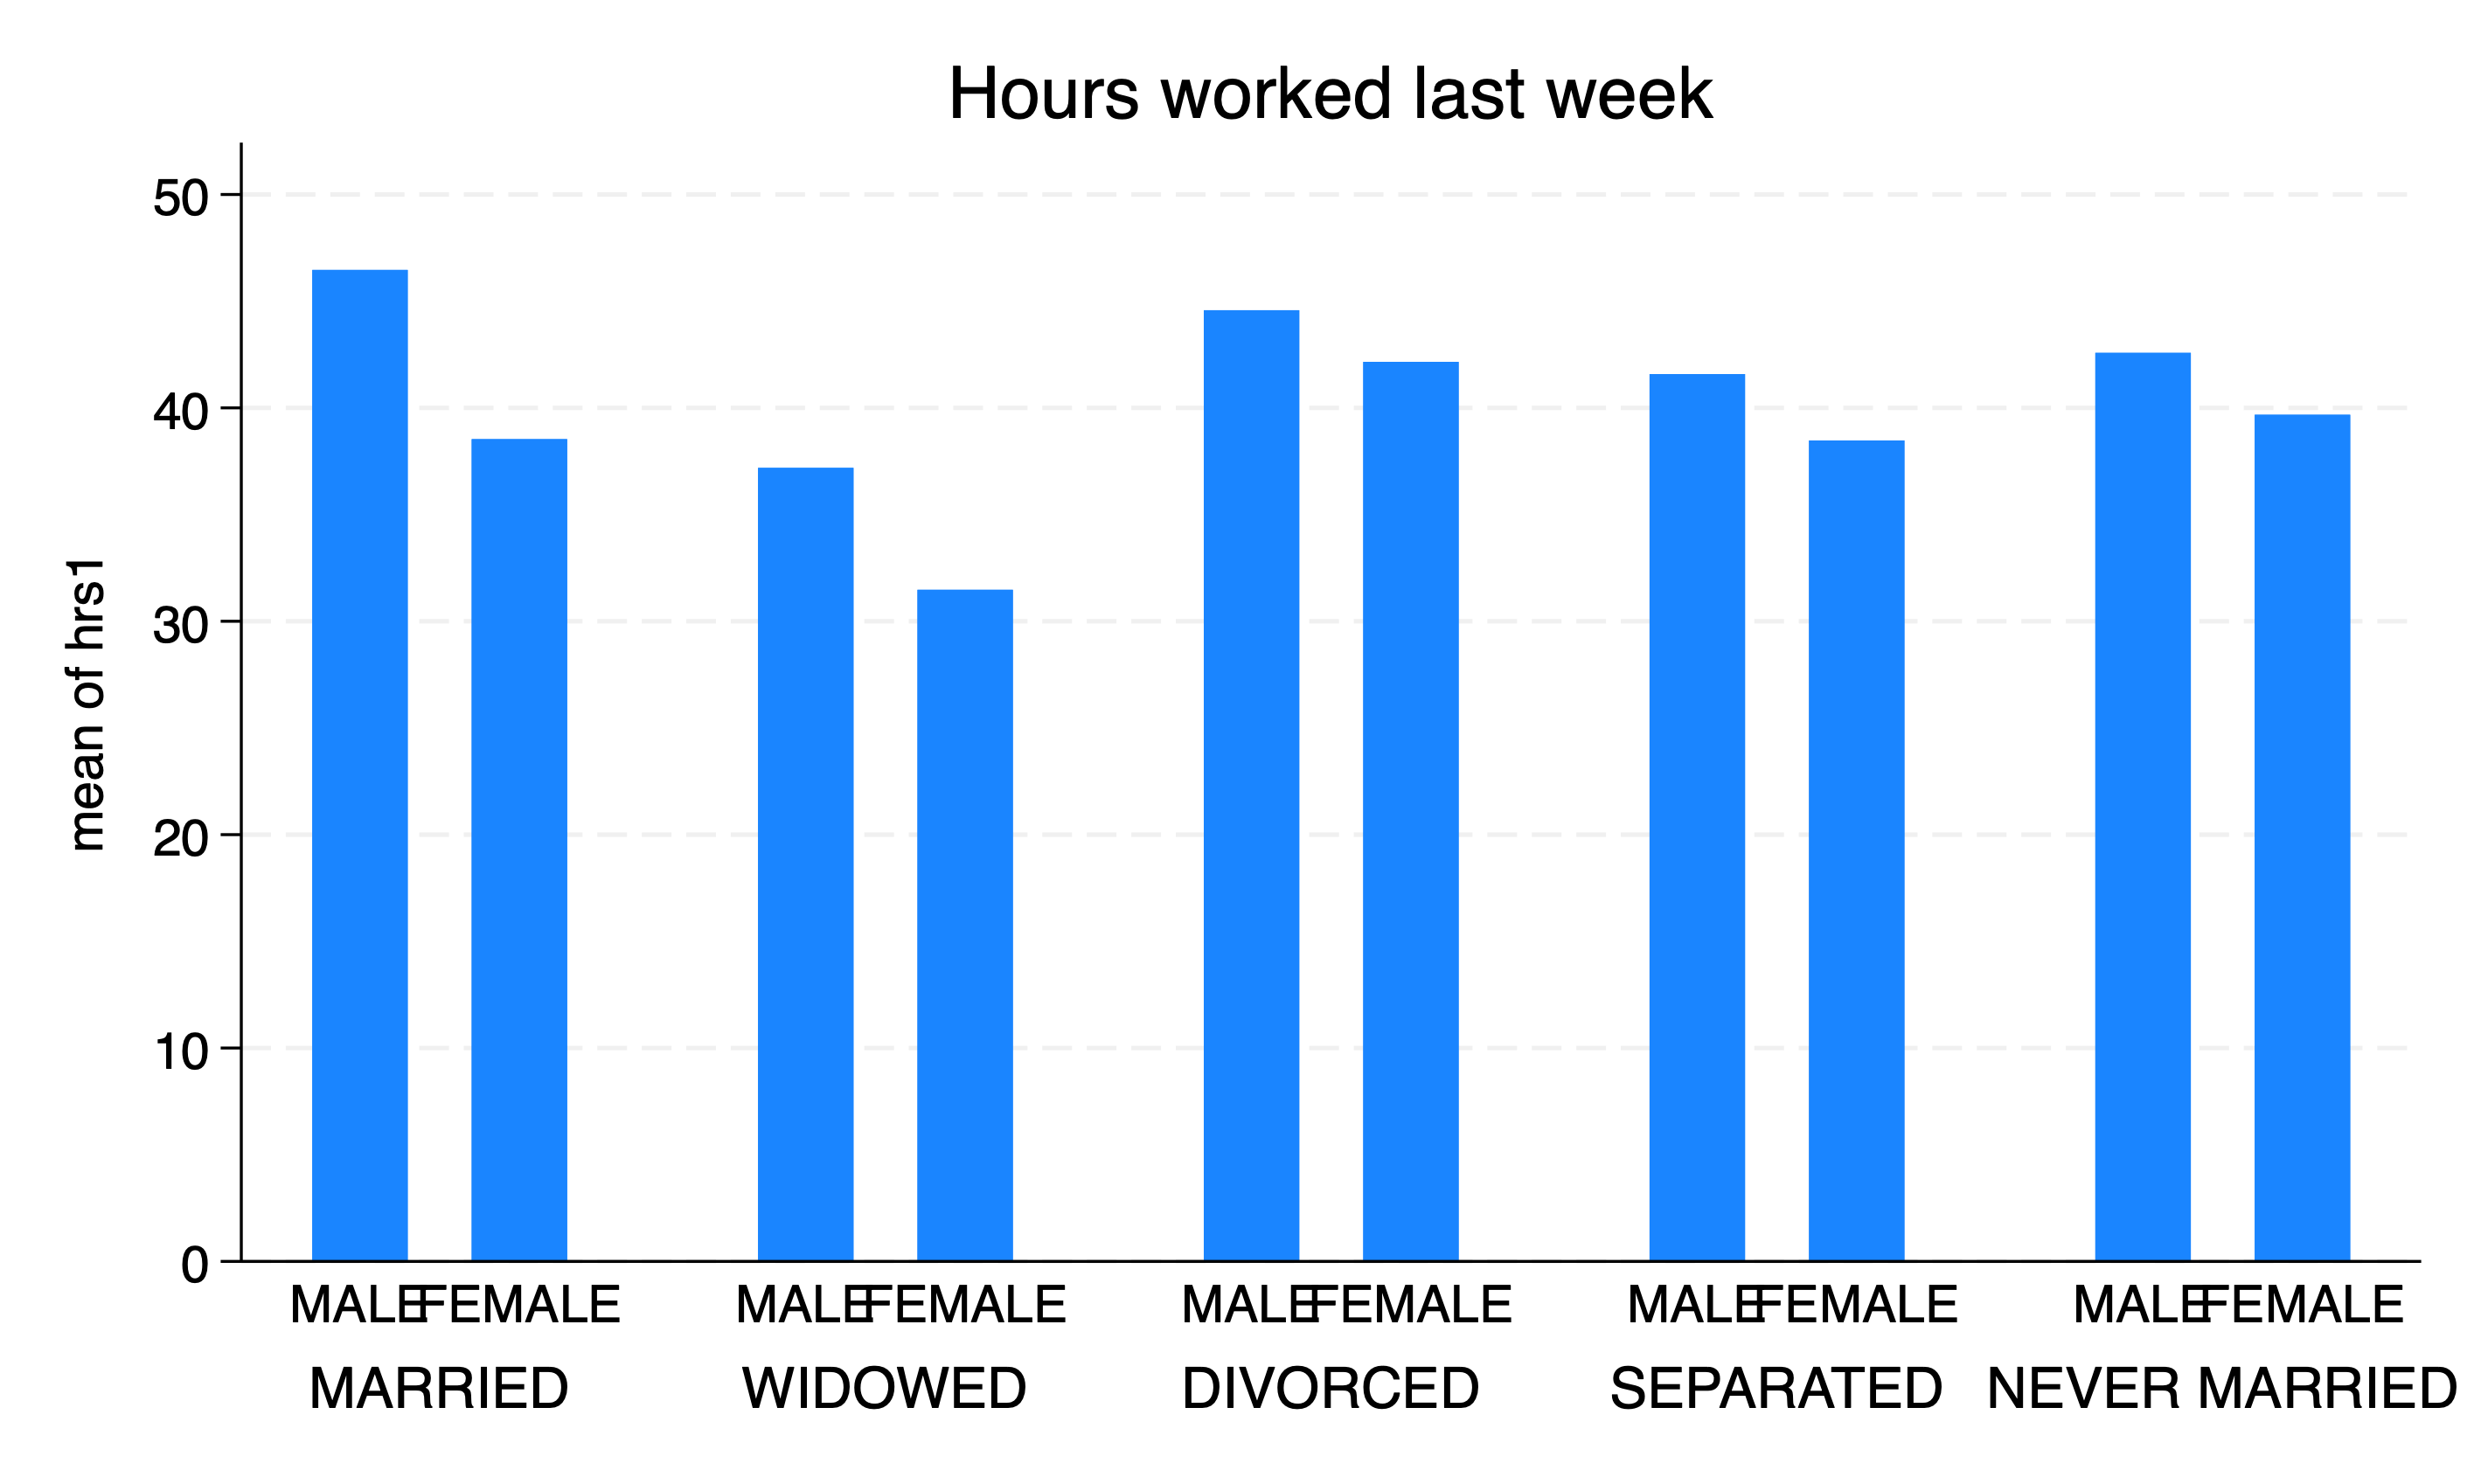
\includegraphics[keepaspectratio,alt={Figure 4.4: Poorly formatted bar chart summarzing hours by sex and marital status}]{week4_barhoursbad.png}}
\caption{Figure 4.4: Poorly formatted bar chart summarzing hours by sex and marital status}
\end{figure}

\[ \]

This does the job, but it does not look very good. We can add some options to improve the format. First, we should add a subtitle to indicate that the means are by sex and marital status with the option \emph{subtitle()}. Next our categorical labels are too big and overlapping. We will edit the option with options within options. For sex, we will edit \emph{over(sex)} by angling the label and making it smaller with \emph{over(sex, label(angle(45) labsize(small)))}. For marital status, we will alternative the labels so they don't overlap and make them smaller with \emph{over(marital,label(alternate labsize(small)))}. Next, we should add a axis title for the y-axis with \emph{ytitle()}.

\begin{Shaded}
\begin{Highlighting}[]
\KeywordTok{graph} \BaseNTok{bar}\NormalTok{ (}\KeywordTok{mean}\NormalTok{) hrs1, }\BaseNTok{over}\NormalTok{(sex,}\KeywordTok{label}\NormalTok{(angle(45) }\BaseNTok{labsize}\NormalTok{(small))) }\CommentTok{///}
  \BaseNTok{over}\NormalTok{(marital,}\KeywordTok{label}\NormalTok{(alternate }\BaseNTok{labsize}\NormalTok{(small))) }\BaseNTok{blabel}\NormalTok{(}\BaseNTok{bar}\NormalTok{, }\KeywordTok{format}\NormalTok{(\%9.1f)) }\CommentTok{///}
  \BaseNTok{title}\NormalTok{(Hours worked }\FunctionTok{last} \FunctionTok{week}\NormalTok{) }\BaseNTok{subtitle}\NormalTok{(}\KeywordTok{by}\NormalTok{ gender and marital status) }\CommentTok{///}
  \DecValTok{scheme}\NormalTok{(s1mono) }\BaseNTok{ytitle}\NormalTok{(}\StringTok{"Mean of Working Hours per Week"}\NormalTok{)}
\end{Highlighting}
\end{Shaded}

\begin{figure}
\centering
\pandocbounded{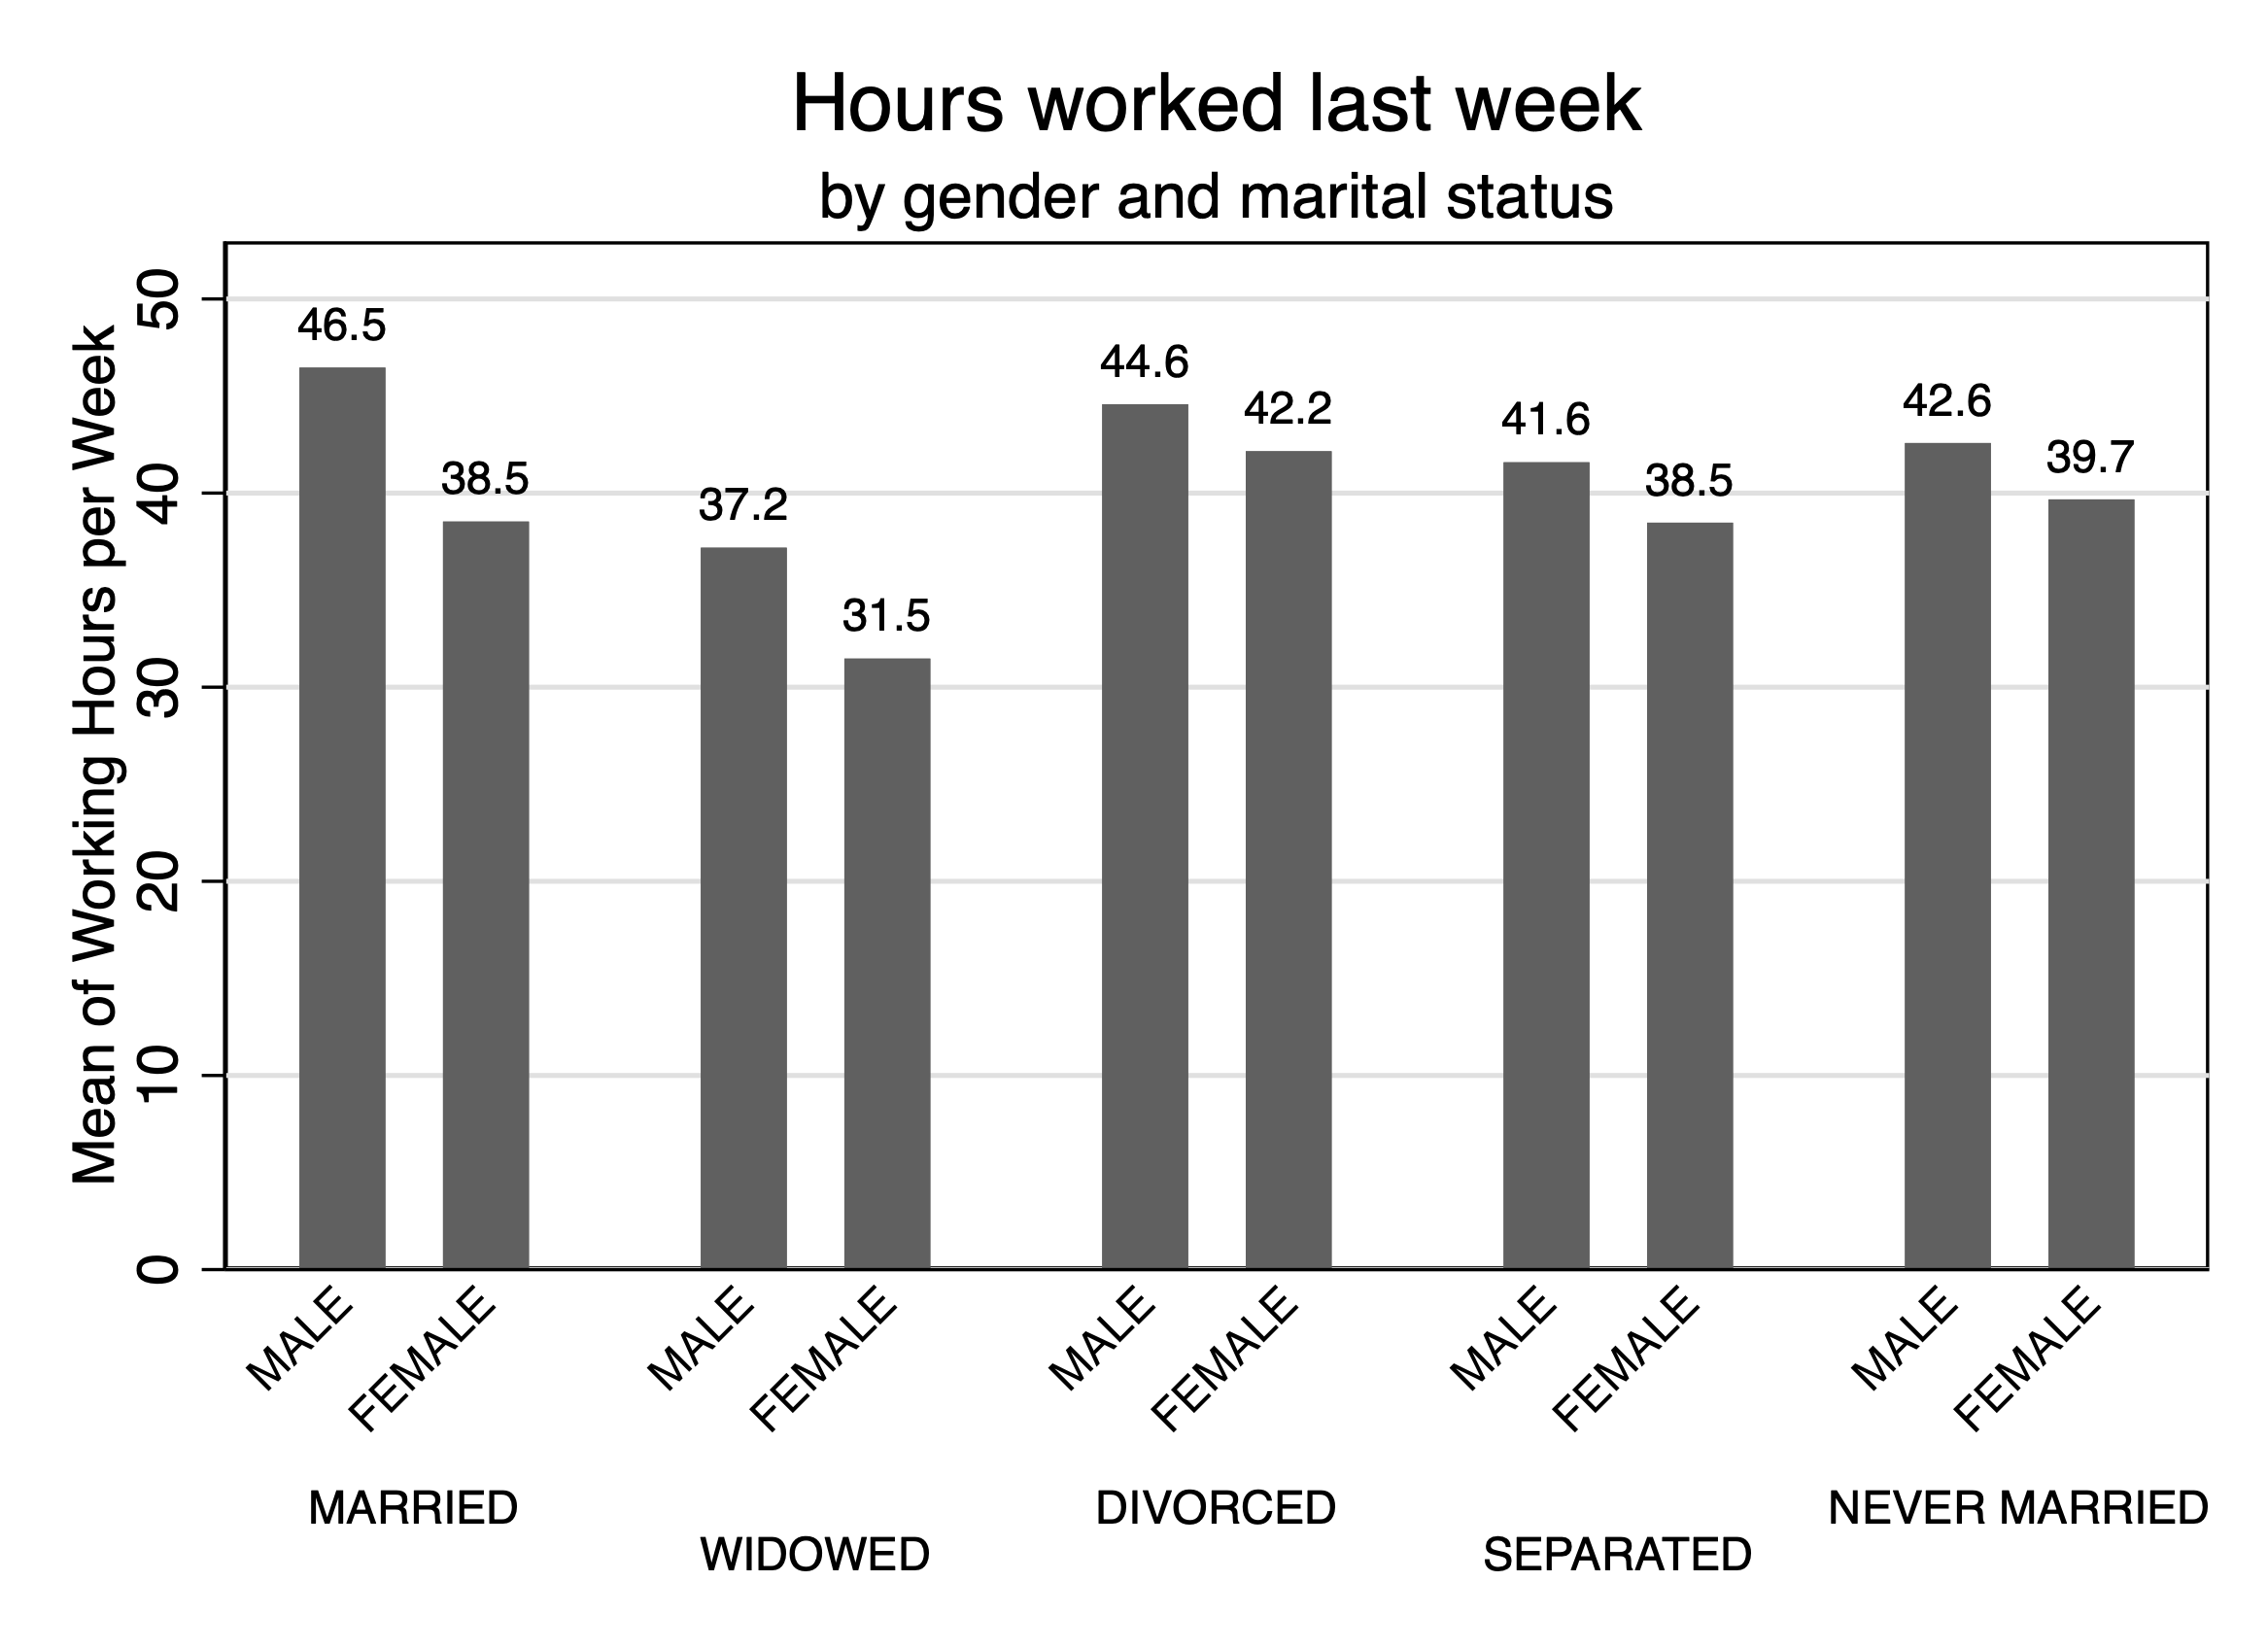
\includegraphics[keepaspectratio,alt={Figure 4.5: Bar chart summarzing a quantitative variable by categories of a nominal variable}]{week4_barhours.png}}
\caption{Figure 4.5: Bar chart summarzing a quantitative variable by categories of a nominal variable}
\end{figure}

\[ \]

This is looking better. I will note that, in my personal opinion, formatting Stata graphics can be a challenge and can have a steep learning curve. My recommendation is finding chart formats that work and work of their code. You will eventually pick up how to format. Stata's help pdf are a great resource, but can be overwhelming for new users at first.

\textbf{Question}: What is missing from this graph given that is a sample from the population?

\section{\texorpdfstring{Power Analysis using \(\chi^2\) test}{Power Analysis using \textbackslash chi\^{}2 test}}\label{power-analysis-using-chi2-test}

We will hop ahead a bit and discuss power analysis. \textbf{Power} is the probability of correctly rejecting a \(H_0\) when it is false (Anderson, et al, 2016). Power is related to our sample size. What is the sample size we need to find statistically significant results?

Acock (2023) takes a randomized subset of 10\% of the 2006 General Social Survey and runs a two-way or cross-tabulation on \emph{sex} and \emph{health}. We will add the option \emph{lrchi2}, which is a likelihood-ratio \(\chi^2\) statistic. We will need this instead of the Pearson \(\chi^2\) statistic.

\begin{Shaded}
\begin{Highlighting}[]
\KeywordTok{use}\NormalTok{ gss2006\_chapter6\_10percent, }\KeywordTok{clear}
\KeywordTok{tabulate}\NormalTok{ sex health, lrchi2 }\OtherTok{row}
\end{Highlighting}
\end{Shaded}

\begin{verbatim}
(General Social Surveys, 1972-2006 [Cumulative File], Dataset 0001)


+----------------+
| Key            |
|----------------|
|   frequency    |
| row percentage |
+----------------+

           |             CONDITION OF HEALTH
    Gender | EXCELLENT       GOOD       FAIR       POOR |     Total
-----------+--------------------------------------------+----------
      MALE |        48         82         32          4 |       166 
           |     28.92      49.40      19.28       2.41 |    100.00 
-----------+--------------------------------------------+----------
    FEMALE |        44         98         43         14 |       199 
           |     22.11      49.25      21.61       7.04 |    100.00 
-----------+--------------------------------------------+----------
     Total |        92        180         75         18 |       365 
           |     25.21      49.32      20.55       4.93 |    100.00 

 Likelihood-ratio chi2(3) =   6.1135   Pr = 0.106
\end{verbatim}

It seems that Men are more likely than women to report being in excellent health, while women are more likely to report being in poor health than men. However, we fail to reject the null hypothesis that they health differs between men and women, since \(Pr=0.106\) which is greater than 0.05.

Note, that we are only using 10\% of the survey. How many observations do we need to find a statistically significant difference (if one exists) between men and women on reporting health?

There is a user-generated command called \emph{chi2power} from Philip Ender that can conduct a power analysis. We need to search for the \emph{chi2power} package in Stata by running the following and installing the package.

\begin{Shaded}
\begin{Highlighting}[]
\KeywordTok{search}\NormalTok{ chi2power}
\end{Highlighting}
\end{Shaded}

In order to run the \emph{chi2power} command, we need to use the \emph{lrchi2} option with the \emph{tabulate} command. We conduct the power analysis by typing the command \emph{chi2power}. Next, we need to provide the options. First, we will use the option \emph{startf(1)}, which means start from 1 times the sample size or \(n=365\). Next, we will use the option \emph{endf(10)}, which means end at 10 or end at \(n=365 \times 10\). Finally, we use the option \emph{incr(1)}, which means increment from 1 to 10 by 1.

\begin{Shaded}
\begin{Highlighting}[]
\NormalTok{chi2power, startf(1) endf(10) incr(1)}
\end{Highlighting}
\end{Shaded}

\begin{verbatim}
alpha = .05
sample size factor = 1.00 power = 0.5265 for n = 365
sample size factor = 2.00 power = 0.8476 for n = 730
sample size factor = 3.00 power = 0.9623 for n = 1095
sample size factor = 4.00 power = 0.9922 for n = 1460
sample size factor = 5.00 power = 0.9986 for n = 1825
sample size factor = 6.00 power = 0.9998 for n = 2190
sample size factor = 7.00 power = 1.0000 for n = 2555
sample size factor = 8.00 power = 1.0000 for n = 2920
sample size factor = 9.00 power = 1.0000 for n = 3285
sample size factor = 10.00 power = 1.0000 for n = 3650
\end{verbatim}

We need power of at least \(0.80\) to find statistically significant results, but researchers prefer a power \(0.90\). Our results show that \(n=365\) then our power is only \(power=0.53\). This means we would obtain a statistically significant \(\chi^2\) about \(52.7\%\) of the time. However, if we double the sample size to \(n=730\) then our power becomes \(power=0.85\). This means we will get a statistically significant \(\chi^2\) \(85\%\) of the time.

Power analysis is important so get an idea of the required sample size for you data collection. If our sample size included 500 observations, our power would be below the threshold of \(80\%\). However, if we collect 2,000 observations, then we an unnecessary and expensive survey. This is an inefficient use of the funds for the analysis.

\chapter{Exercises}\label{exercises}

\section{General Social Survey}\label{general-social-survey}

\subsection{Explanatory and Outcomes}\label{explanatory-and-outcomes}

Steps

\begin{enumerate}
\def\labelenumi{\arabic{enumi}.}
\tightlist
\item
  Use the file gss2006\_chapter6.dta
\item
  Our variables of focus will be \emph{sex} and \emph{premars}
\item
  Let's answer the question: Do men and women have different views on premarital sex?
\item
  Which variable is the explanatory/independent variable?
\item
  Which variable is the outcome/dependent variable?
\item
  Run a \emph{tabulate} command. We want to include conditional percentage \(P(Opinion|Men)\) and \(P(Opinion | Women)\)
\item
  Calculate a \(\chi^2\) statistics.
\item
  Do you find a statistically significant difference?
\item
  Calculate a Cramer's V.
\item
  What do you find about the relationship?
\item
  Interpret the conditional percentage.
\end{enumerate}

\subsection{Categorical and Quantitative Variables}\label{categorical-and-quantitative-variables}

Steps

\begin{enumerate}
\def\labelenumi{\arabic{enumi}.}
\tightlist
\item
  Use the file gss2006\_chapter6.dta
\item
  We are interested in the differences in average weekly working hours \emph{hrs1} by political views \emph{polviews}.
\item
  Use the \emph{table} command to find the mean, standard deviation, and frequency by political views.
\item
  Do you find any differences? How do the extreme ends compare?
\item
  Create a bar chart using \emph{graph bar (mean) hrs1}. Add labels to the bars and use the options to format.
\end{enumerate}

\section{Ordinal Variables}\label{ordinal-variables}

Steps

\begin{enumerate}
\def\labelenumi{\arabic{enumi}.}
\tightlist
\item
  Use the file gss2006\_chapter6.dta from AGIS
\item
  We are intered in the variables \emph{polviews} and \emph{premars}
\item
  Do political views explain premartial sex opinions?
\item
  Use the \emph{tabulate} command to do a two-way tabulation or cross-tabulation
\item
  Add the appropriate option to find conditional percentages for \(P(Opinion | PolitcalView)\)
\item
  Add the test statistic options for \(\chi^2\), Cramer's \(V\), and \(\tau_b\).
\item
  What do you conclude?
\item
  What is the strength of the relationship?
\item
  Interpret the conditional percentages.
\end{enumerate}

\section{Current Population Survey}\label{current-population-survey}

Steps

\begin{enumerate}
\def\labelenumi{\arabic{enumi}.}
\tightlist
\item
  Let's use the NBER CPS Merged Outgoing Rotation Group (MORG) data extraction
\item
  The data can be directly downloaded from: \url{https://data.nber.org/morg/annual/morg24.dta}
\item
  Please review the data dictionary: \url{https://data.nber.org/morg/docs/cpsx.pdf}
\end{enumerate}

\subsection{Nominal and Quantitative Variables}\label{nominal-and-quantitative-variables}

Steps

\begin{enumerate}
\def\labelenumi{\arabic{enumi}.}
\tightlist
\item
  What is the difference in earnings between union members and non-union members?
\item
  Our variables of interest are \emph{unionmme} and \emph{earnwke}.
\item
  Use the \emph{table} command to compare means, standard deviations, and frequencies of weekly earnings between union members and non-union members
\item
  Use the \emph{bar graph (mean)} to display differences in means between union members and non-union members.
\end{enumerate}

\section{Nominal Variables}\label{nominal-variables}

Steps

\begin{enumerate}
\def\labelenumi{\arabic{enumi}.}
\tightlist
\item
  Use the NBER CPS MORG data extraction
\item
  Is there a relationship between \emph{sex} and laborforce status \emph{lfsr94}?
\item
  Use the \emph{tabulate} command to calculate conditional percentages.
\item
  Use the options for calculating the \(\chi^2\) and Cramer's \(V\).
\item
  Interpret your results.
\item
  Who is more likely to report being employed?
\end{enumerate}

Acock, A.C. (2023). A gentle introduction to Stata. 6th ed.~Stata Press.

Anderson, D. R., Sweeney, D. J., Williams, T. A., Camm, J. D., \& Cochran, J. J. (2016). Statistics for business and economics (13th ed.). Cengage Learning.

Mitchell, M. N. (2020). Data management using Stata: A practical handbook. Stata Press.

\bibliography{book.bib,packages.bib}

\end{document}
